\documentclass[10pt]{article}
\usepackage{icmlko}

\icmlmeta{IP 파운데이션 월드모델}{336}{읽는 쪽}{같은 결정이 세 층에 새겨져 있었다 --- 거르는 쪽 · 긁는 쪽 · 그리고 읽는 쪽}

\begin{document}

\twocolumn[
\icmlheader

\begin{abstract}
노트 333이 만화 · 세계애니 검색이 0\%인 것을 ``게으름''이라 부르고 다
긁었다. \textbf{긁고 나니 여전히 0\% 였다.} \texttt{lab/trendaxes.FILE} 에
그 두 도메인이 \emph{없었다}. \texttt{ingest/trend\_all.SPEC} 에는 있다 ---
\textbf{쓰는 쪽과 읽는 쪽이 갈라져 있었다.} 노트 149 때(검색 0\%) 만들어진
목록이 노트 237(데이터랩은 영문 질의를 받는다) 뒤에도 안 고쳐졌고,
\textbf{아무도 안 긁었으니 티가 안 났다.}

\textbf{같은 결정이 세 층에 새겨져 있었다} --- 거르는 쪽(\texttt{idol\_axes}
한터 필터 · 노트 326) · 긁는 쪽(\texttt{wiki\_views} · \texttt{album\_meta} ·
노트 332 · 333) · \textbf{읽는 쪽}(\texttt{trendaxes.FILE} · 오늘).

두 줄을 더하고 다 긁었다. \textbf{만화 1,473건 중 실제 계열은 73건(5\%) ·
세계애니 1,311건 중 241건(18\%)}이다. 빈 계열을 0 으로 세는 현행 규약
(\texttt{zero\_is\_data=True})에서는 축 덮음이 만화 \textbf{53.7\%} ·
세계애니 \textbf{63.7\%} 가 된다.

\textbf{판은 못 가른다} --- 짝지어(학습 재추출 열둘) $-$0.0024(SD 0.0047 ·
3/12)로 미결정 폭 0.010 안이다. 그런데 \textbf{자기 도메인은 번다}:
세계애니 \textbf{$+$0.0046(10/12)} · 웹툰 $+$0.0032(9/12) · 팝업
$+$0.0311(10/12). 그리고 \textbf{작은 도메인은 잃는다}: 도서
$-$0.0233(2/12) · 시장팝업 $-$0.0359 · 아이돌 $-$0.0194.

\textbf{크기 법칙은 안 선다} --- 유보 수와 차의 상관이 $+$0.358($p{=}0.31$)
이고 팝업(유보 59)이 제일 크게 벌었다. \textbf{작은 데가 잃는 것은 맞는데
크기로는 못 예측한다.}
\end{abstract}
]

\section{쓰는 쪽과 읽는 쪽}

\begin{center}\footnotesize
\begin{tabular}{lll}
\hline
층 & 어디 & 무엇 \\
\hline
거르는 쪽 & \texttt{ingest/idol\_axes} & 한터 필터(326) \\
긁는 쪽 & \texttt{wiki\_views} & 축 파일을 읽음(332) \\
 & \texttt{idol\_album\_meta} & 필터 복사(333) \\
\textbf{읽는 쪽} & \texttt{lab/trendaxes.FILE} & \textbf{두 도메인 없음} \\
\hline
\end{tabular}
\end{center}

\textbf{셋 다 ``나중에 고칠 자리''를 안 고친 것이다.} 그런데 셋이 서로를
가려 준다 --- 안 긁으니 읽는 쪽이 비어 있어도 모르고, 읽는 쪽이 비어 있으니
긁어도 안 붙는다. \textbf{노트 333에서 만화를 긁고 ``5\%뿐''이라 적었을 때
사실은 붙지도 않고 있었다.}

\begin{figure*}[t]
\centering
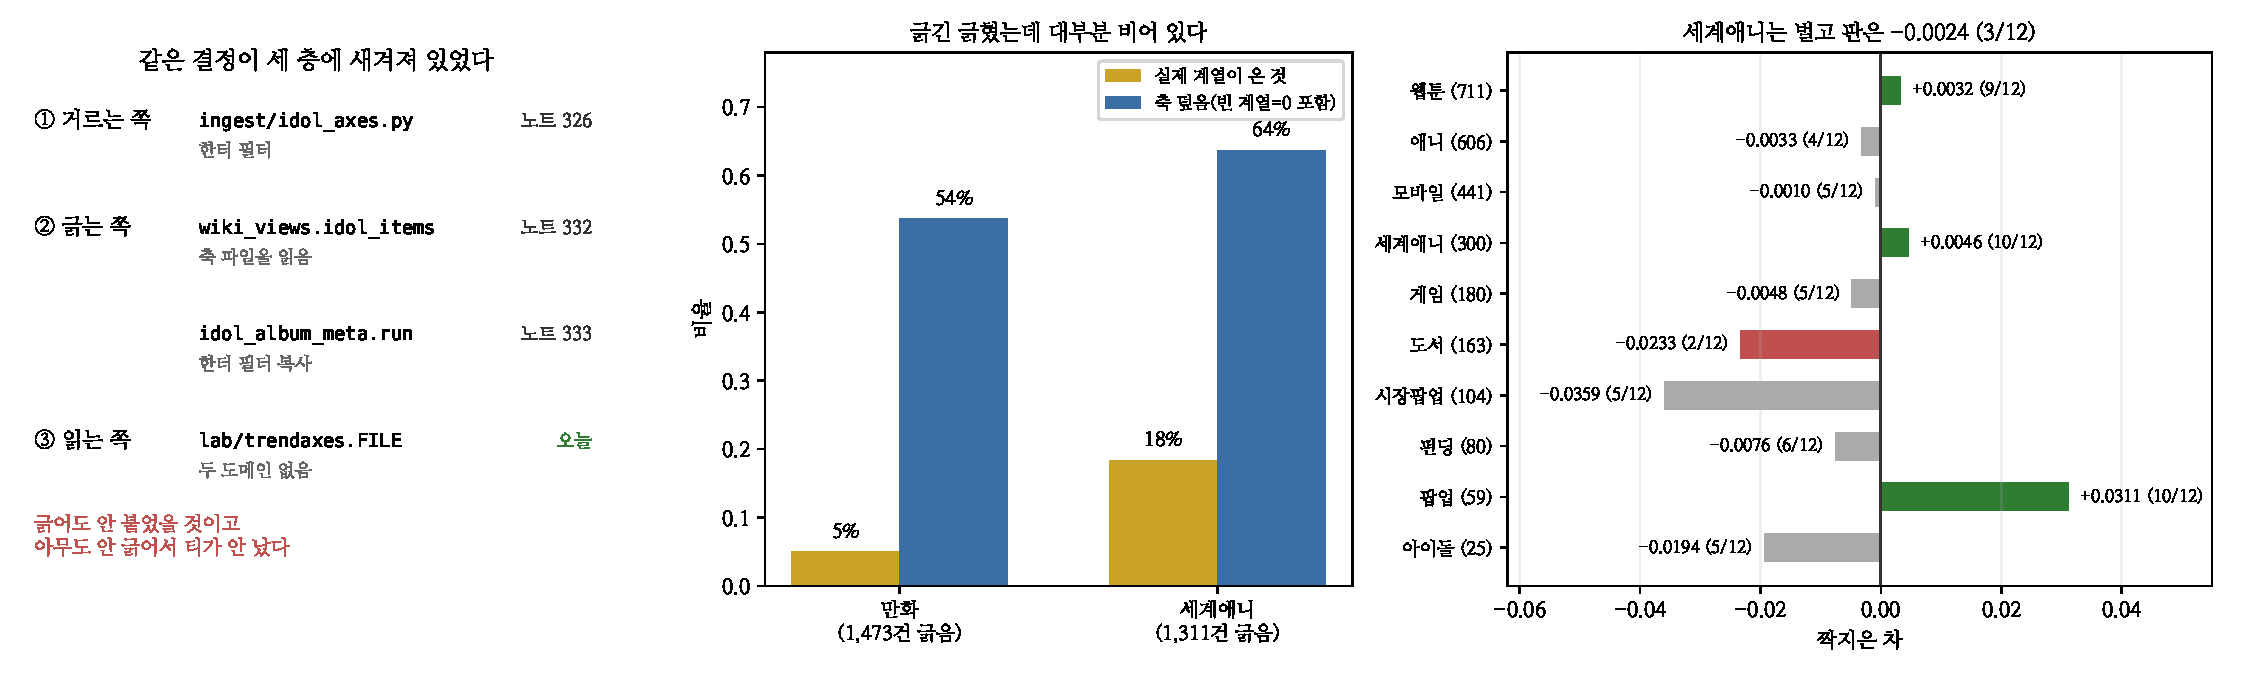
\includegraphics[width=\textwidth]{figs/reading.pdf}
\caption{왼쪽 --- 세 층. 가운데 --- 긁은 것과 붙은 것.
오른쪽 --- 도메인별 짝지은 차.}
\end{figure*}

\section{긁긴 긁혔는데 대부분 비어 있다}

\begin{center}\footnotesize
\begin{tabular}{lrrr}
\hline
 & 긁은 것 & 실제 계열 & 축 덮음 \\
\hline
만화 & 1,473 & 73 (5\%) & 53.7\% \\
세계애니 & 1,311 & 241 (18\%) & 63.7\% \\
\hline
\end{tabular}
\end{center}

차이는 \texttt{zero\_is\_data=True} 다 --- 물어봤는데 빈 계열이 온 것을
``아무도 안 찾았다''로 읽어 0 으로 넣는다. \textbf{그 규약이 이 두
도메인에서 덮음의 대부분을 만든다}(만화는 54\%p 중 49\%p가 0 이다).

\section{판은 못 가르고 자기 도메인은 번다}

\begin{center}\footnotesize
\begin{tabular}{lrrr}
\hline
도메인 & 유보 & 짝지은 차 & 양수 \\
\hline
웹툰 & 711 & $+$0.0032 & 9/12 \\
애니 & 606 & $-$0.0033 & 4/12 \\
모바일 & 441 & $-$0.0010 & 5/12 \\
\textbf{세계애니} & 300 & \textbf{$+$0.0046} & \textbf{10/12} \\
게임 & 180 & $-$0.0048 & 5/12 \\
도서 & 163 & $-$0.0233 & 2/12 \\
시장팝업 & 104 & $-$0.0359 & 5/12 \\
펀딩 & 80 & $-$0.0076 & 6/12 \\
\textbf{팝업} & 59 & \textbf{$+$0.0311} & \textbf{10/12} \\
아이돌 & 25 & $-$0.0194 & 5/12 \\
\hline
\textbf{판} & 2,675 & \textbf{$-$0.0024} & 3/12 \\
\hline
\end{tabular}
\end{center}

\textbf{만화는 유보 6행이라 채점에서 빠진다} --- 학습에만 기여한다. 그래서
이 처치의 채점 쪽 효과는 사실상 세계애니 하나다.

\paragraph{왜 남이 잃나} 검색은 \emph{공유} 축이라 다른 도메인에 열이
늘지 않는다 --- 노트 335의 열 비용이 아니다. 바뀌는 것은 \textbf{풀의
구성}이다. 만화 961행 · 세계애니 1,878행에 검색 값이 생기면서 풀린
계수가 움직인다. 노트 329가 ``남의 뽑기가 내 점수를 흔든다''를 잰 그
통로다.

\section{남은 것}
\begin{center}\footnotesize
\begin{tabular}{ll}
\hline
갈래 & 왜 \\
\hline
\texttt{zero\_is\_data} 를 갈라 & 0 이 절반인데 자료인가 \\
\textbf{목록 둘을 대조} & 다른 축에도 갈라진 것이 있나 \\
세계애니 $+$0.005 를 승격 & 판은 $-$0.002 라 못 가른다 \\
팝업이 왜 $+$0.031 인가 & 유보 59행인데 제일 많이 벌었다 \\
\hline
\end{tabular}
\end{center}

\paragraph{규약} \textbf{목록이 둘이면 언젠가 갈라진다.} 무엇을 긁을지의
목록(\texttt{ingest/trend\_all.SPEC})과 무엇을 읽을지의 목록
(\texttt{lab/trendaxes.FILE})이 따로 있었고, 한쪽만 고쳐진 채로 노트 백 편이
지나갔다. \textbf{그리고 갈라진 것이 조용했다} --- 덮음 0\% 는 ``자료가
없다''로 읽혔지 ``목록이 다르다''로 안 읽혔다. 노트 149가 그 0\% 를 근거로
위키 축을 만들었고 그 판단은 결과적으로 옳았지만, \textbf{근거는 반쯤
틀린 것이었다.} 도메인을 새로 열 때 ``이 도메인이 \emph{모든} 목록에
들어 있나''를 한 번 세어야 한다.

\end{document}
